\hypertarget{prompting-analysis}{\subsection{Prompting analysis}}
\label{sec:prompting-analysis}
While the benchmark we design is general, we evaluate \nummodels models by adapting them through few-shot prompting (see \refsec{prompting}).
Consequently, here we study variations across several of these models with respect to different design decisions involved in prompting.\footnote{We do not conduct all of these analyses on every model due to cost. We exclude all commercial models due to monetary cost, as well as TNLGv2 models due to long wait times given the scale of the model.}
Together, these analyses help clarify the potential brittleness of model behavior to prompt design, which bears on the legitimacy and reliability of using prompting to build practical systems.

\paragraph{Choice of in-context examples.}
Given that we adapt language models through few-shot prompting, the selection of the specific in-context examples could significantly influence model performance.
In particular, unlike prior work \citep[\eg][]{brown2020gpt3}, we use the same examples across all evaluation instances, rather than selecting different in-context examples for each evaluation instance, as this better reflects the realities of few-shot adaptation \citep{perez2021true}.
(We describe our specific selection algorithm which, to first-approximation, is random selection from the scenario's training set while ensuring coverage of different classes for classification problems, in \refsec{prompting-remainder}.)
As a consequence, this exacerbates the variation observed for different choices of in-context examples (consistent with the high variability one might witness in practice if they truly only have a few examples). 

To measure this sensitivity, we repeat all evaluations for \numruns runs, meaning \numruns choices of the in-context examples.
To explore the sensitivity of model results to this choice, hover over a specific entry to see the variance across runs on the website.
Further, the predictions across the \numruns runs can be found for a given evaluation instance.
Additionally, we visualize the accuracy range (best minus worst performance) across seeds in \reffig{seed-variance}.
We observe that the performance of most models tends to be relatively consistent: the median range (across scenarios) is below 0.03 for 24 out of 28 models (exceptions are \yalm, \gptdavinci, \gptcurie, \gptada).
Interestingly, we find that there are scenarios where all models tend to exhibit higher variance.
A prominent example is \naturalquestions (open-book), where the median range is 0.1730 (e.g., \gptdavinci obtains F1 scores of 0.376, 0.611, and 0.636 across the three sets of in-context examples).

\begin{figure}
\centering
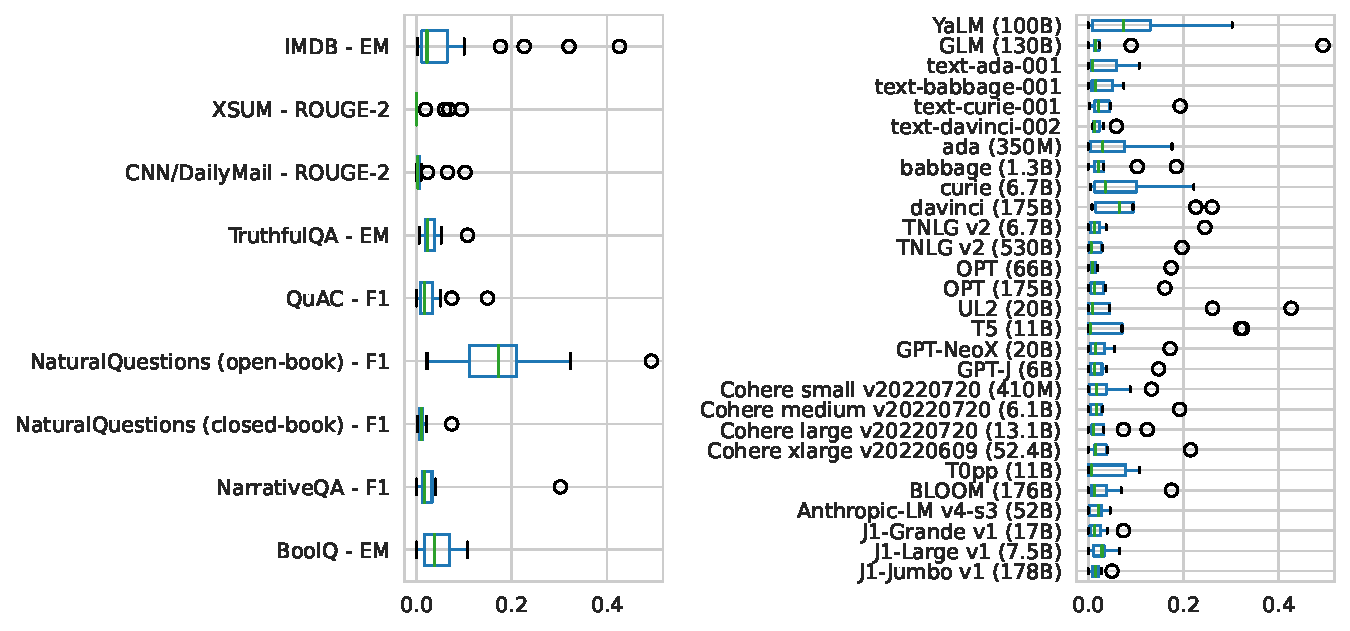
\includegraphics[width=\textwidth]{plots/seed_variance.pdf}
  \caption{\textbf{Variance across seeds.} 
    For a subset of models and scenarios, we evaluate each scenario with three different random sets of in-context examples.
    We compute the range of the accuracy metric (maximum minus minimum value over the three random seeds) and visualize across models and scenarios.
  }
  \label{fig:seed-variance}
\end{figure}

\paragraph{Number of in-context examples.}
By default, we either use \numincontext in-context examples, or fewer examples for scenarios where \numincontext examples do not fit within in the context window. 
To test how the number of examples (\ie the sample efficiency of adaptation) influences performance, we vary the maximum number of examples across $n \in \{0, 1, 2, 4, 8, 16\}$.
In \reffig{in-context-ablations}, we plot model performance as a fraction of the average number of in-context examples provided (which may be fewer than the maximum stated above if they do not fit inside the context window).
To explore the results further, including the model generations, see  \benchmarkUrlPrefix{ablation\_in\_context}.

\begin{figure}
\centering
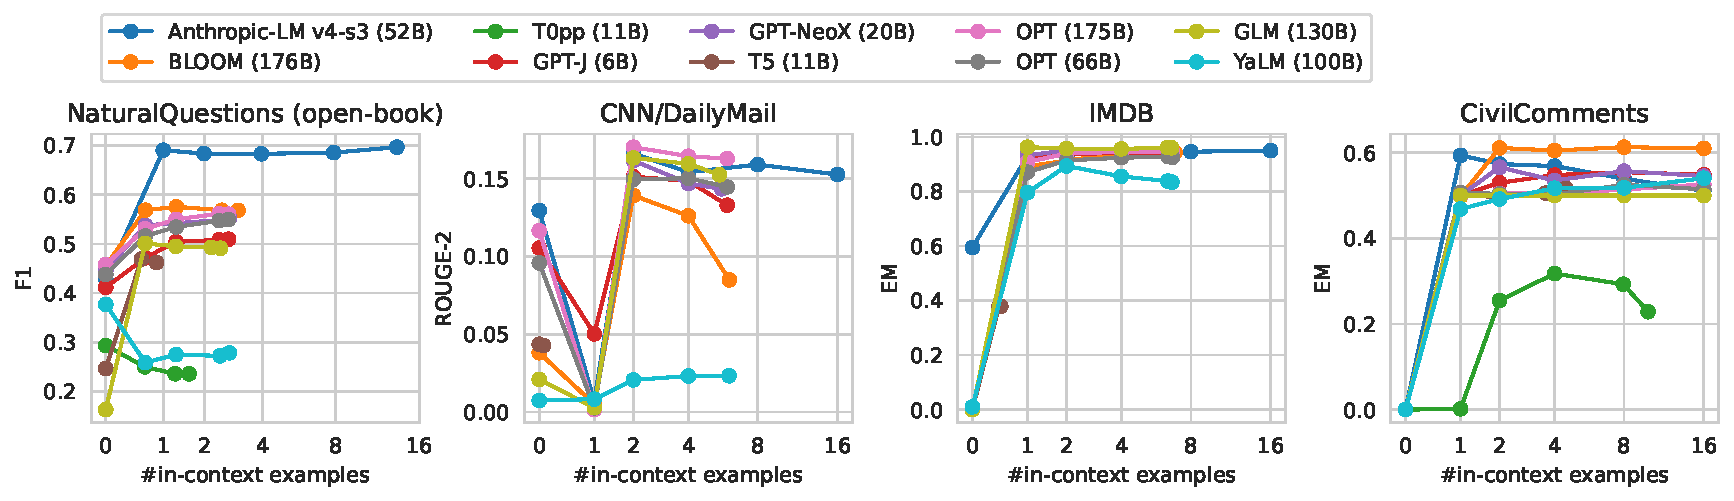
\includegraphics[width=\textwidth]{plots/in_context_ablations.pdf}
  \caption{\textbf{Number of in-context examples.} 
    For each model, we set the maximum number of in-context examples to [0, 1, 2, 4, 8, 16] and fit as many in-context examples as possible within the context window.
    We plot performance as a function of the average number of in-context examples actually used.
  }
  \label{fig:in-context-ablations}
\end{figure}

We find that all models show clear improvement from $n = 0$ to $n = 1$, sometimes having 0\% accuracy in the zero-shot setting, with the consistent exception of \cnndm where zero-shot accuracy is better for almost all models.
% Removed for TMLR
% This aligns with our analyses in \refsec{human-evaluation-summarization}, in 
% Added for TMLR
We posit
that models may not effectively understand the appropriate length distribution and the poor reference summaries may comparatively mislead the model in the one-shot setting compared to the zero-shot setting.
However, for larger numbers of in-context examples, we do not see consistent benefits across all models and all scenarios.
The sole exception is \optonesevenfive which, besides \cnndm, shows a perfectly monotonically increasing relationship between number of shots and model accuracy for \naturalquestions (open-book), \imdb, and \civilcomments.

\paragraph{Formatting of prompt.}
As we describe in \refsec{prompting}, beyond the in-context examples and the evaluation instance, there are several other details required to fully specify a prompt (\eg instructions that describe what the model should do).
Since this formatting exists in the space of natural language, it is difficult to specify concrete axes to systematically vary across (\ie in contrast to how we can specify a range we consider for the number of in-context examples).
Consequently, we consider the following motivated but fairly \textit{ad hoc}/arbitrary changes to the prompt format involving instructions, input prefixes, output prefixes, and input suffixes. The exact changes to the prompt can be found at \benchmarkUrlPrefix{ablation\_prompts}, along with the results.

\begin{figure}
\centering
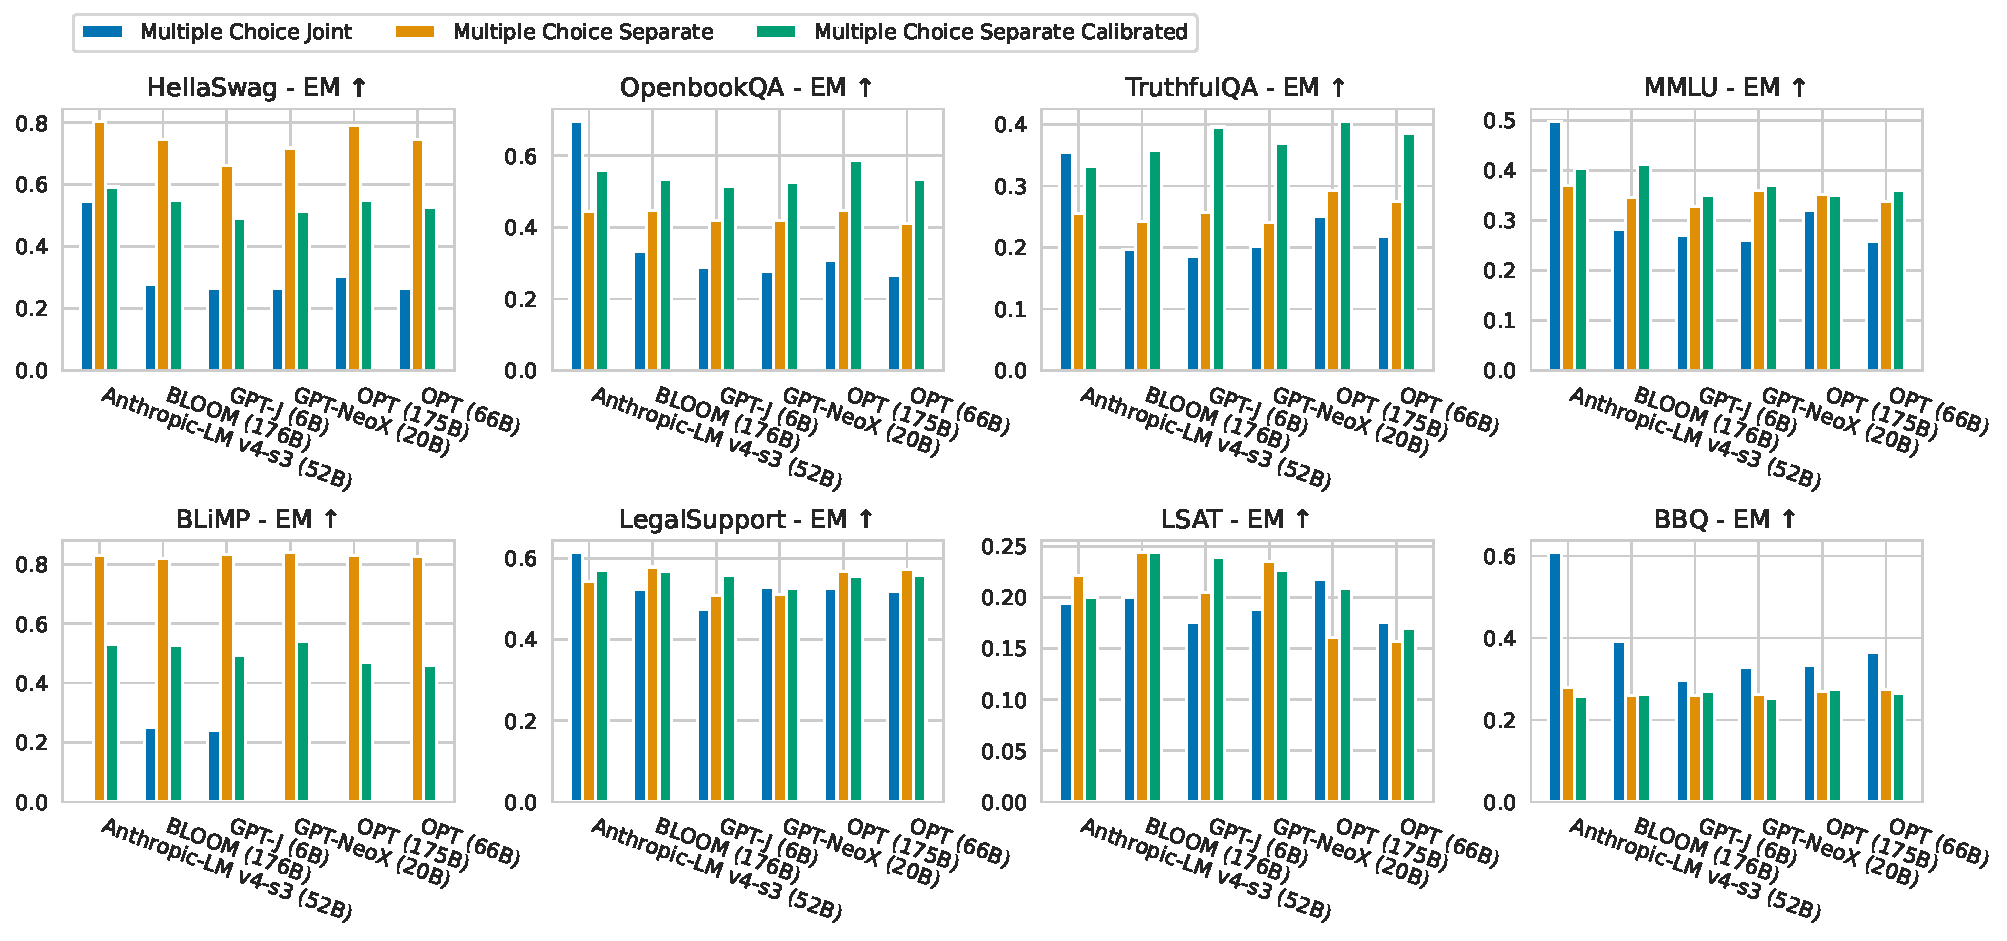
\includegraphics[width=\textwidth]{plots/mc_ablations.pdf}
  \caption{\textbf{Multiple-choice adaptation.} 
    For each adaptation method (joint, separate, and separate calibrated), we compare models across scenarios.
  }
  \label{fig:mc-ablations}
\end{figure}

The clear finding is that the best prompt formatting is not consistent across models (\ie models can stand to improve in their interoperability).
In particular, one variants lead to an accuracy of 67.3\% for \anthropic on \naturalquestions (open-book), whereas the prompt performs very poorly for \bloom, which drops from an accuracy around 60\% to 8.5\%. 
In some cases, we believe the prompting changes may lead to poor/undesirable interactions with the tokenizer, given the models use different tokenizers in several cases. 
For \glm, we are intrigued to see the prompt involving mentioning the model is an expert AI assistant performs best across all four scenarios (\naturalquestions (open-book), \cnndm, \imdb, and \civilcomments) we look in terms of accuracy.
Specifically, the prompt includes \texttt{instructions} of  ``I am an expert AI assistant who is here to help you with the following.'', along with an \texttt{input\_prefix} of ``Passage: '',  \texttt{input\_suffix} of `` "'', and an \texttt{output\_prefix} of ``Answer:''

\paragraph{Formulation of multiple choice scenarios.}
Beyond the details of the prompt, we can conceptually imagine different ways to make use of the language interface to perform the same underlying scenario.
As we discuss in \refapp{adaptation}, in the case of multiple choice scenarios, we could provide the model with all of the answer choices and task it with selecting the correct choice (\textit{joint}).
Or we could provide the model with each answer choice as a separate query of the model, and see which answer choice is assigned higher probability (\textit{separate}).
And we could further calibrate the model-assigned probabilities by the probability the model assigns to the corresponding answer choice when presented standalone (\textit{separate-calibrated}).

The results for these multiple choice scenarios as a function of this choice can be found at \benchmarkUrlPrefix{ablation\_multiple\_choice}, and they are visualized in \reffig{mc-ablations}.
We observe that the method that maximizes accuracy is largely determined by the scenario, whereas it is generally consistent across models for a given scenario.
Taking \hellaswag as a case study, for all six models, the methods follow \textit{separate} $>$ \textit{separate-calibrated} $>$ \textit{joint}.
This choice can be very consequential for the model accuracy: for \optonesevenfive, the accuracies are 79.1\%, 54.8\%, and 30.2\% respectively. 
Further, the trends are entirely inverted for calibration error, as may be expected.
So, overall for \hellaswag, across both desiderata and for all six models, there is clear and strict Pareto dominance in adaptation methods of \textit{separate} $>$ \textit{separate-calibrated} $>$ \textit{joint}.
In the case of \hellaswag, given the dataset is designed as completions of an incomplete textual sequence, the preference for the \textit{separate} adaption method over the \textit{joint} adaptation method is fairly intuitive and precisely aligns with the empirical findings. 
However, we do note the methods pattern differently for specific models in terms of efficiency.
In particular, the \textit{separate} methods require a query for each answer choice, whereas the \textit{joint} method requires a single, much longer (especially due to the inclusion of in-context examples) query.
This manifests in lower denoised inference times for \textit{separate} over \textit{joint} for \bloom (0.075s vs. 0.271s), but the opposite trend for \optonesevenfive (0.71s vs. 0.187s), despite the fact the models are evaluated on the same infrastructure and are near-identical in overall parameter count.

For the other scenarios, we do not observe as model-agnostic preferences over the adaptation methods.
In general, for accuracy, we find \textit{separate-calibrated} $>$ \textit{separate} $>$ \textit{joint} for \openbookqa, \truthfulqa, and \mmlu for five of the six models.
The consistent exception is \anthropic where the preference is consistently \textit{joint} $>$ \textit{separate-calibrated} $>$ \textit{separate}.
We find this to be quite striking: the adaptation method that elicits the most accurate behavior from \anthropic elicits the least accurate behavior from the other five models.
These gaps are significant as well: on \openbookqa, presenting accuracies in the order (\textit{separate-calibrated}, \textit{separate}, \textit{joint}), we see (58.6\%, 44.6\%, 30.9\%) for \optonesevenfive, whereas for \anthropic we see (55.8\%, 44.4\%, 69.6\%).
That is, if \optonesevenfive and \anthropic were compared using the \textit{separate-calibrated} adaptation method (or the \textit{separate} method), they would achieve near-equal accuracies (within 3\%), but they are almost 40\% apart when using the \textit{joint} method, and 12\% apart when comparing the per-model accuracy-maximizing method.
This raises fundamental questions about the appropriate way to compare across models and the sense in which uniform standardization is fair; we encourage future work to more extensively look into this and develop clearer best practices.